\section{ПРОЕКТИРОВАНИЕ ПРОГРАММНЫХ МОДУЛЕЙ}
\label{sec:theory}

\subsection{Постановка задачи проекта}
\label{sub:theory:goals}
Основной целью данного проекта является разработка программного продукта для интеграции трехмерной модели в веб-среду,
манипуляции трехмерной геометрией и загрузкой/выгрузкой трехмерной модели в файл.

Основные требования к разрабатываемой системе:
\begin{itemize}
\item Возможность отображения трехмерной модели в веб-документе
\item Возможность манипуляции трехмерной моделью в трехмерном пространстве (применение трех фундаментальных операций -- трансляция, поворот и масштабирование) 
\item Возможность загрузки трехмерной модели из файла стандартизированного формата (*.obj, *.blend)
\item Возможность выгрузки трехмерной модели в файл для последующего открытия (*.obj)
\end{itemize}

В качестве платформы для разработки
приложения избран веб-фреймворк Reactjs ввиду высокой совместимости его компонентной модели с полностью функциональной
парадигмой разработки - Redux, которая хорошо подходит для реализации приложения для редактирования пользовательского
контента.

За основной механизм отображения принята комбинация WebGL + HTML5 canvas, позволяющая интегрировать трехмерную графику в
веб-документ.

Для реализации вышеуказанного функционала не требуется централизованного сервиса или хранилища, поэтому приложение может быть
размещено в среде статического HTML веб-сайта, например на github.io pages. Для добавления коммерческого функционала и расширения и
улучшения существующего допустима реализация централизованного веб-сервера или кластера серверов для обработки высокопроизводительных
задач, таких как рендеринг сложных сцен в высоком разрешении (в условиях, когда ресурсы клиентского компьютера ограничены).

В качестве основного языка разработки приложения используется язык TypeScript, потому как он дает разработчикам возможность писать строготипизированный код,
проверяемый на этапе компиляции, что уменьшает необходимость покрытия некоторого тривиального кода системы модульными тестами для обеспечения типовой безопасности
во время выполнения приложения.

\subsection{Язык TypeScript}
\label{sub:theory:typescript}

TypeScript --- язык программирования с открытым исходным кодом, разрабатываемый и поддерживаемый Microsoft Corporation. Является более строгим надмножеством языка JavaScript
и добавляет опциональные элементы статической типизации и основанную на механизме классов (в отличие от механизма прототипов для Native JavaScript) реализацию объектно-ориентированной парадигмы.
Данный язык, являясь надстройкой над JS, может использоваться для разработки как клиентских приложений для выполнения в браузере, так и серверных для выполнения в таких средах,
как Node.js или JSX. \cite{typescript1}\cite{typescript2}

Среди основных отличий языка от Native JavaScript можно отметить следующие особенности:
\begin{itemize}
\item типовые аннотации для функций и членов классов;
\item файлы объявлений;
\item классы и интерфейсы;
\item generic-типы;
\item модули и пространства имен;
\item смешения (Mixin);
\item типы-перечисления;
\item инструкция \textit{await};
\item кортежи.
\end{itemize}

Основное назначение языка - упрощение разработки более крупных клиентских приложений, добавление механизмов статической типизации, позволяющих избежать большого количества
простых ошибок на этапе транскомпиляции, которые могли бы повлиять на выполнение кода во время работы программы. Тем не менее, поскольку статическая типизация является
опциональной (однако, ее можно установить принудительно посредством некоторых флагов компиляции, таких как --noImplicitAny), все программы, написанные на Native JavaScript,
также являются валидными TypeScript программами. Это обеспечивает обратную совместимость и простую миграцию для legacy-проектов. Разработчики TypeScript искали решение,
которое не будет нарушать совместимость со стандартом и его кросс-платформенной поддержкой. Зная, что только стандарт ECMAScript предлагает поддержку в будущем для
программирования на базе классов (Class-based programming), TypeScript был основан на этом предположении. Это привело к созданию компилятора JavaScript с набором
синтаксических языковых расширений, увеличенным на основе предложения, которое трансформирует расширения в JavaScript. В этом смысле TypeScript является представлением
того, что ожидать от ECMAScript 6 (рисунок \ref{fig:theory:typescript:typescript}). Уникальный аспект не в предложении, а в добавлении в TypeScript статической типизации,
что позволяет статически анализировать язык, облегчая оснастки и IDE поддержку.

\begin{figure}[ht]
\centering
  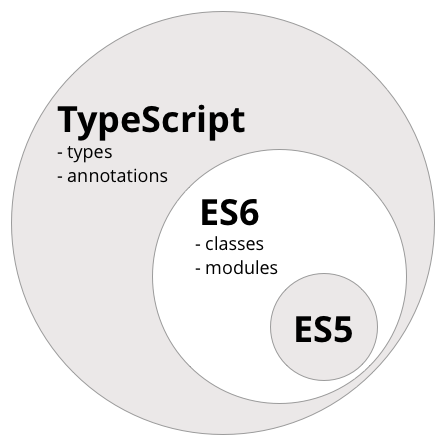
\includegraphics[scale=0.6]{typescript.png}
  \caption{Функционал языка TypeScript}
  \label{fig:theory:typescript:typescript}
\end{figure}

Одним из результатов работы TypeScript компилятора является набор так называемых typing-файлов, имеющих расширение *.d.ts. Данные файлы - вспомогательные для
компилятора и являются метаданными модулей и классов, компилируемых TypeScript. Ближайшим аналогом данных файлов являются *.h и *.hpp файлы языков C/C++. Данные
typing-файлы хранят информацию о публичном интерфейсе генерируемых классов и являются <<клеем>>, связывающим сгенерированные *.js файлы с исходными *.ts и *.tsx файлами.

Статический анализ typing-файлов позволяет реализовать механизм подсказок и автодополнение кода в IDE, поддерживающих TypeScript. Среди самых распространенных
можно отметить следующие IDE:
\begin{itemize}
\item Atom Text Editor с плагином Typed --- основной текстовый редактор, используемый в данной дипломной работе;
\item Visual Studio 2013 Update 2 и позже;
\item GNU Emacs с плагином <<Company>>.
\end{itemize}

Для автоматизации процесса транскомпиляции TypeScript целесообразно использовать так называемые <<Task-runner>> программы, такие как <<Grunt>> или <<Gulp>>.
Использование оных позволяет подписаться на события изменения файлов исходного кода проекта и перекомпилировать проект в JavaScript по мере изменения исходного
кода в автоматическом режиме. Для настройки данных инструментов используются Gruntfile либо Gulpfile (в зависимости от избранного Task-runner). Эти файлы,
являясь аналогами GNU Makefile, есть ни что иное как скрипты для компиляции, определяющие конвеер, обрабатывающий все файлы в проекте по мере их модификации.
Реализация данных файлов на ранних этапах разработки проекта позволяет повысить степени автоматизации и легко внедрить такие инструменты разработки, как
средства продолжительной интеграции, автоматизированное тестирование и версионирование исходного кода.


\subsection{Компонентное проектирование системы}
\label{sub:theory:components}
Веб-приложение, использующее аппаратную графику, имеет несколько иную структуру, нежели классическое веб-приложение ввиду его разделение на две уединенные части -- часть,
отвечающую за отображение пользовательского интерфейса в HTML (часть, пресущую всем веб-приложениям), и часть отображения трехмерной графики (рисунок \ref{figure:theory:webgl_app}).
Разрабатываемая система подразделяется на компоненты исходя из их целевого назначения и разные компоненты имеют строго уединенные зависимости.

\begin{figure}[ht]
\centering
  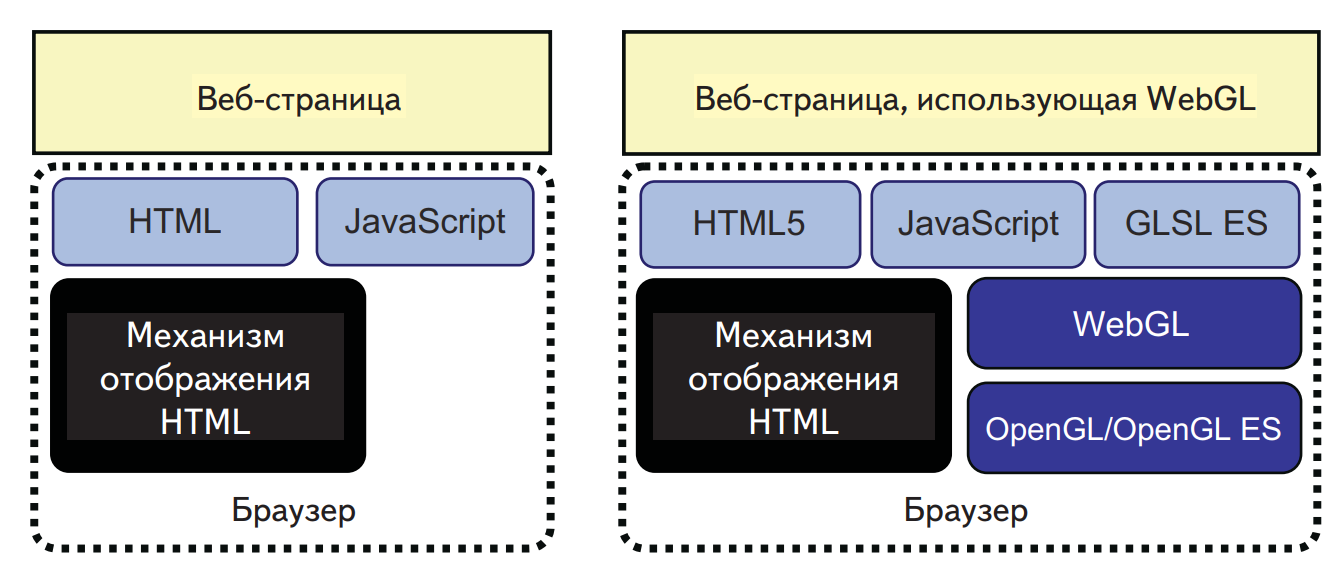
\includegraphics[scale=0.35]{web_with_webgl.png}
  \caption{Отличие приложения для отображения трехмерой графики от классического веб-приложения.}
  \label{figure:theory:webgl_app}
\end{figure}

Типичная модель приложения, производящего CRUD-операции (Cre-ate, Read, Update, Delete) обычно содержит в себе набор связанных между собой модулей,
имеющих строго определенные на этапе компиляции связи. Поскольку разрабатываемая система является частным случаем CRUD-системы (без возможности удаления
пользовательского содержимого), то схожая декомпозиция системы может быть применена и для нее. Разрабатываемая система условно подразделяется на следущие модули:

\subsubsection{Компонент отображения}
\label{sub:theory:components:rendering}

Основное назначение компонента отображения -- собственно вызов низкоуровневых API WebGL, итерация по вершинам трехмерной модели и их добавление в контекст
отображения WebGL. Также данный компонент служит для контроля над материалами и шейдерами для отображения различных элементов трехмерной модели.
Данный компонент имеет зависимость от стороннего модуля threejs, который упаковывается вместе с остальными сторонними библиотеками и подключается к
приложению динамически.

Основные части компонента отображения:

\begin{itemize}
\item CanvasRenderer -- модуль, занимающийся непосредственной манипуляцией вершинами трехмерной модели при ее отображении.
\item MaterialPicker -- модуль-описатель свойств материалов, содержит в себе описания всех шейдеров, необходимых для отображения материалов.
\item GeometryIterator -- модуль, предназначенный для итерации по вершинам трехмерной модели для последующего отображения его в CanvasRen-derer.
\end{itemize}

Публичный интерфейс компонента состоит из следующих методов:
\begin{itemize}
\item setRenderingModel(modelInfo) -- устанавливает модель для отображения из информации о модели. Аргумент modelInfo -- объект-описатель геометрии отображаемого объекта;
\item render(cameraInfo) -- непосредственно отображает модель на canvas. Аргумент cameraInfo -- трансформ-сущность камеры (ее положение в пространстве и поворот), тип камеры (орто, перспектива);
\item clearScreen() -- очищает экран.
\end{itemize}

\subsubsection{Компонент геометрических вычислений}
\label{sub:theory:components:calculation}

Основное назначение компонента геометрических вычислений -- произведение функциональных манипуляций над точками в трехмерном пространстве, преобразования вершин трехмерной модели, применение
фундаментальных трансформаций к точкам (трансляция, поворот, масштабирование) и реализация вспомогательных математических операций для работы с трехмерной сценой. Данный компонент имеет стороннюю
зависимость от стандартной библиотеки математики JavaScript.Math и от модуля underscore (lodash) для функциональной работы с коллекциями данных и векторами.

Основные части компонента графических вычислений:

\begin{itemize}
\item VectorTranslator -- модуль, реализующий операцию трансляции векторов. Использует библиотеки векторной манипуляции underscore, lodash;
\item VectorRotator -- модуль, реализующий операцию поворота вектора на определенный угол относительно определенной оси. Реализует операции поворота с помощью кватернионов;
\item VectorScaler -- модуль, реализующий операцию масштабирования вектора относительно начала координат или другой произвольной точки;
\item QuaternionHelper -- вспомогательный модуль реализующий арифметические операции над кватернионами и трехмерными векторами. Используется в VectorRotator и является частью публичного интерфейса
данного компонента;
\item VectorHelper -- вспомогательный модуль, реализующий арифметические операции над трехмерными векторами. Используется во всех подсистемах компонента графических вычислений и также является частью 
публичного интерфейса данного компонента;
\item VectorProjector -- модуль-аггрегатор поведения других модулей, реализующих стандартные операции. Реализует преобразования проекций трехмерной модели до отображения ее на экране.
\end{itemize}

Публичный интерфейс компонента состоит из следующих методов и вспомогательных типов:
\begin{itemize}
\item класс VectorHelper -- реализующий армифметику над векторами;
\item класс QuaternionHelper -- реализующий армифметику над кватернионами и векторами;
\item performMVProjection(model, camera) -- реализует проецирование трехмерной модели из пространства сцены в пространство камеры.
\end{itemize}

\subsubsection{Компонент пользовательского интерфейса}
\label{sub:theory:components:ui}

Основное назначение компонента пользовательского интерфейса (Компонента UI) -- реализация возможностей по манипулации состоянием приложения для пользователя, оргазинация
контрольных элементов для вызова функций приложения.
Компонент UI отвечает за управление пользовательским интерфейсом системы и содержит ряд интерфейсов-контрактов и классов для взаимодействия с прочими компонентами
с большой степенью абстракции. Компонент UI предоставляет внешним модулям интерфейс \texttt{IUIDisplayable}, объявляющий метод обязанный реализовать набор правил
по установлению связи между доменной абстракцией системы и объектом, являющимся его моделью отображения.

Компонент UI будучи точной входа в React-приложение (и в приложение в целом), имеет большое число вспомогательных модулей, поэтому перечисление их всех не представляется целесообразным.
Следует также обратить внимание на тот факт, что в терминах Reactjs, модули пользовательского интерфейса также именуются компонентами, что вносит некоторую двусмысленность в перечисление списка
подмодулей компонента UI. Далее в этом списке под компонентом имеются в виду React-компоненты. Фактически, в рамках компонента реализуется модуль на каждый элемент пользовательского 
интерфейса, такой как кнопка или элемент меню. Ниже представлены основные элементы данного компонента:

\begin{itemize}
\item AppComponent -- фактическая точка входа в приложение, является объектом вызова ReactDOM.render и контейнером всех остальных систем.
\item BasicOperationsComponent -- дочерний к AppComponent элемент, является контейнером элементов пользовательского интерфейса, отвечающих за вызов базовых преобразований трехмерной
модели -- трансляции, поворота и масштабирования.
\item MainMenuComponent -- дочерний к AppComponent элемент, реализующий стандартное меню приложения и доступ к глобальным базовым функциям приложения (например, загрузка и выгрузка моделей).
\end{itemize}

Данный компонент является де-факто Main модулем приложения, что означает, что все зависимости на диаграмме компонентов направлены от него. Данный компонент содержит основной тип-точку входа
приложения, выраженную в типе AppComponent. Являясь React-компонентов, AppCompo-nent встраивается в DOM веб-страницы и управляет состоянием отображения всего приложения, выстраивая иерархическую структуру
компонентов.

Тем не менее, компонент UI предоставляет набор публичных интерфейсов для того, чтобы обеспечить соблюдение принципа обращения зависимостей (D -- Dependency Inversion в SOLID\cite{solid}).
Данные публичные интерфейсы предназначены для организации сильной типизации и статического анализа связи компонентов и реализации архитектуры приложения в стиле набора плагинов для основного,
так называемого Main-модуля.

Публичный интерфейс, предоставляемый компонентом UI будет иметь следующий вид:
\begin{itemize}
\item event onUpdateGUIState(newState) -- метод-обработчик события, означающий, что необходимо обновление состояния определенного компонента пользовательского
интерфейса. newState -- аргумент-описатель нового события системы, на основании которого произведится обновление.
\item event onNewModel -- метод-обработчик события создания новой модели (другие компоненты системы могут подписываться на обработку этого события).
\item event onModelLoaded(modelInfo) -- обработчик события выбора существующей модели, сохраненной для дальнейшего использования в локальном хранилище приложения, modelInfo --
метаинформация о выбранной на пользовательском интерфейсе модели.
\end{itemize}


\subsubsection{Компонент обработки геометрии}
\label{sub:theory:components:geometry}

Основное назначение компонента обработки геометрии - работа со структурами данных, описывающими трехмерные модели, реализация логики по манипуляции трехмерной геометрией,
основных операций при редактрировании моделей -- подразделения и выталкивания, методы оптимизации моделей -- удаление лишних вершин и треугольников.
Данный компонент реализует ключевые абстракции системы, такие как ModelGeometryInfo -- описатель геометрии трехмерной модели, аггрегирующий в себе информацию о положении вершин модели
в модельном пространстве, а так же информацию о соединении вершин в треугольники. CameraInfo -- описатель положения и поворота камеры и другие важные абстрации.

Основные модули компонента обработки геометрии:
\begin{itemize}
\item класс ModelGeometryInfo -- хранилище двух списков Vector[] vertices и number[] triangles. Описывает геометрию трехмерного объекта и содержит координаты каждой из вершин модели в
модельном пространстве а также группы по три индекса вершин, составляющих единый треугольник.
\item класс ModelLoopExtruder -- тип, реализующий стратегию выталкивания определенных вершин модели поперек замкнутой цепочки вершин -- одну из стандартных операций редактора трехмерных моделей.
\item класс ModelGeometrySubdivider -- тип, реализующий стратегию подразделения модели для увеличения числа треугольников и увеличения ее детализации -- одну из стандартных операци создания
трехмерной модели из примитива.
\item класс VertexGeometryHelper -- тип-утилита, реализующая функционал для работы с полигонами и вершинами модели, позволяя найти полигоны, соседствующие с полигоном или вершины, соседствующие
с вершиной. Данный тип используется всеми другими типами данного компонента, однако предоставляется в общий доступ для сторонних использований.
\end{itemize}

Публичный интерфейс данного компонента представляет из себя набор методов для манипуляции структурами данных:
\begin{itemize}
\item getExtruderFor(modelInfo) -- предоставляет реализацию типа Model-LoopExtruder, сконфигурированную для данной модели. Является методом фабрикой, предназначенной для использования в других
частях системы (например, в компоненте пользовательского интерфейса, внутри обработчика событий по манипуляции моделью).
\item getSubdividerFor(modelInfo) -- предоставляет реализацию типа Model-GeometrySubdivider, сконфигурированную для данной модели. Является методом фабрикой, предназначенной для использования в других
частях системы (например, в компоненте пользовательского интерфейса, внутри обработчика событий по манипуляции моделью).
\item getSubdividerFor(modelInfo) -- предоставляет реализацию типа Vertex-GeometryHelper, сконфигурированную для данной модели. Является методом фабрикой, предназначенной для использования в других
частях системы (например, в компоненте пользовательского интерфейса, внутри обработчика событий по манипуляции моделью).
\end{itemize}


\subsubsection{Компонент хранения}
\label{sub:theory:components:persistance}

Основное назначение компонента хранения данных состоит в сохранении состояния сессии использования приложения между перезапусками, хранении пользовательских настроек без необходимости доступа к
удаленному серверу, кешировании данных о трехмерных моделях в их бинарном виде при выгрузке модели из области работы и для реализации оффлайн-доступа к системе.
Поскольку в первой версии разрабатываемой системы не подразумевается возможности кросс-клиентского сохранения данных, что означает что при смене клиента (компьютера или иного устройства доступа),
контекст выполнения приложения не будет сохранен, основным механизмом длительного хранения данных в приложении выступает механизм браузера Local Storage.

Однако для сохранения возможностей по расширяемости приложения следует ввести дополнительный слой абстракции (в виде абстрактного класса либо интерфейса). Это позволит дореализовать более
централизованный механизм синхронизации в дальнейшем и соблюсти принцип Открытости-Закрытости (Open-Closed или O в SOLID). Принцип Открытости-Закрытости заключается в такой реализации
компонентов системы, чтобы реализация дополнительного функционала производилась без модификации самих компонентов, а путем внедрения новых компонентов и изменения конфигурации системы для того чтобы
этот функционал задействовать. В случае с компонентом хранилища, реализован абстрактный слой доступа к данным -- асинхронный интерфейс IMo-delDataRepository

 \begin{lstlisting}[language=TypeScript, label=lst:domain:html]
    /// #!/usr/env/node
    /// Target=ES2016

    const Promise = import 'promise'

    default export interaface IModelDataRepository
    {
        /// Async data retrieval operation.
        public async getModelData(modelId: string): Promise<ModelGeometryInfo>;

        /// Async data storage operation.
        public async storeModelData(geometry: ModelGeometryInfo, modelId: strning): Promise<void>;

        /// Async data retrieval operation. Lists all the items in the storage.
        public async listAllModelData(): Promise<ModelGeometryInfo[]>;

        /// Updates the 'last modified' date on the model info storage item.
        public async touchModelData(modelId: strning): Promise<void>;
    }
\end{lstlisting}

Поскольку данный интерфейс является полностью асинхронным (резульатами выполнения всех операций выступает Promise-объект), не составляет труда реализация данного интерфейса, работающая, например, с
сетевым (потому асинхронным) транспортным уровнем, либо чтение из синхронных источников, например из cookie-объектов или localStorage. 

Основные модули компонента хранения:
\begin{itemize}
\item Базовый интерфейс IRepository, являющийся родительским для всех интерфейсов-репозиториев
\item Интерфейс IModelDataRepository
\item Класс LocalStorageModelDataRepository, реализующий интерфейс I-ModelDataRepository. Является асинхронной реализацией, построенной на основе синхронного доступа к Browser Local Storage.
\item Интерфейс IUserSettingsDataRepository
\item Класс LocalStorageUserSettingsDataRepository, реализующий интерфейс IUserSettingsDataRepository. Реализует асинхронный доступ к пользовательским настройскам (предпочитаемый размер окна,
горячие клавиши и т.д.)
\item Интерфейс ICompiledShaderCache
\item Класс LocalStorageCompiledShaderCache, реализующий операции доступа к прекомпилированным шейдерам для различных материалов в трехмерной модели.
\item Интерфейс IConfigurationProvider, реализующий чтение конфигурации приложения, необходимой для работы метода-фабрики (опционального инстанциирования репозиториев).
\end{itemize}

Публичный интерфейс данного компонента представляет из себя набор интерфейсов и методов-фабрик, реализующих инстанциирование экземпляров классов, реализующих данные интерфейсы:
\begin{itemize}
\item Интерфейс IRepository
\item Интерфейс IModelDataRepository
\item Интерфейс IUserSettingsDataRepository
\item Интерфейс ICompiledShaderCache
\item метод-фабрика getInstanceFor<T>(), где T является дочерним к интерфейсу маркеру IRepository
\end{itemize}

\subsection{Реализация асинхронности в приложении}
\label{sub:theory:promise}

Асинхронность компонента хранения достигается за счет использования объектов-обещаний (Promise), по своей природе являющихся указателями на длительную асинхронную операцию. 

Механизм работы объекта обещания изображен на рисунке \ref{fig:theory:promise} и состоит в следующем:

\begin{enumerate}[label=\arabic*.]
\item{Объект <<потребитель>> вызывает <<сервис>> с целью получить некоторые данные либо вызвать удаленный API, ответ от которого может занять неопределенное время.}
\item{Сервис создает объект типа \texttt{Promise<T>}, где \texttt{T} -- тип ожидаемого потребителем значения (может быть \texttt{void}).}
\item{Конструктор типа \texttt{Promise<T>} принимает в качестве аргумента функцию сигнатуры \texttt{(resolve: (T) => void, reject: (any) => void) => void}. Внутри данной функции, сервис
обращается к долгоработающему API (<<сторонний сервис>>) -- это может быть unmanaged-код, управляемый системой сигналов или другой сервис. Единственным требованием к долгоработающему API
является наличие некоторго механзма оповещения о завершении операции. Например, вызов callback-функции или некоторого сигнала.)}
\item{После начала длительной операции и возвращения объекта типа \texttt{Pro- mise<T>}, <<Потребитель>> продолжает свою работу, ожидая ответа от результата длительного вызова. Данные
действия производятся синхронно старту длительной операции. Объект потребитель может делать другие долгие вызовы, обращаться к другим сервисам и т.д.}
\item{После того как все синхронные операции завершатся, поток, обрабатывающий поведение объекта потребителя завершит работать и выйдет за пределы области пользовательского кода,
виртуальная машина языка JavaScript начнет ожидать очередного события в очереди. Рано или поздно, от <<стороннего сервиса>> придет ответ и будет вызвана callback-функция либо сработает
сигнал, который будет воспринят <<сервисом>>.}
\item{Контроль будет передан callback-функции <<сервиса>>, которая либо вызовет функцию \texttt{resolve: (T) => void} с некоторым результатом операции в качестве аргумента,
сигнализируя объекту-обещанию о том, что долгоработающая операция завершилась успешно и были получены данные типа T, либо функцию \texttt{reject: (any) => void}, сигнализирующая
об ошибке. Во втором случае, может быть передан описатель ошибки любого типа и <<потребитель>> может обработать ее соответствующим образом.}
\item{Вызов \texttt{resolve} или \texttt{reject} вызывает обработчики, зарегистрированные объектом <<потребитель>>, тем самым возобновляя процесс выполнения программы.}
\end{enumerate}

\begin{figure}[ht]
\centering
  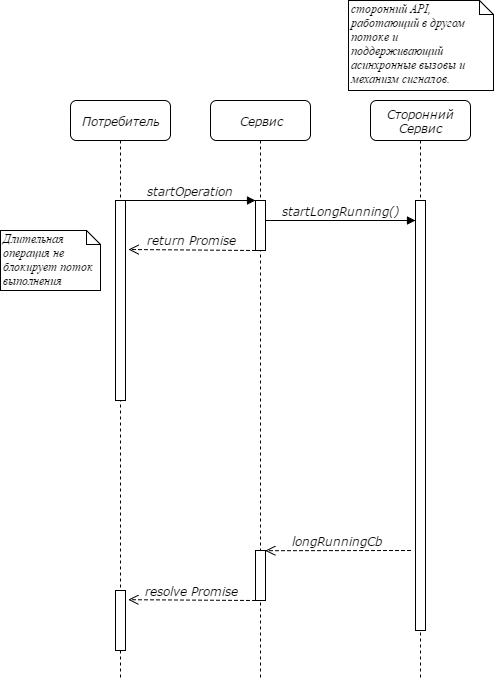
\includegraphics[scale=0.75]{promise.png}
  \caption{Диаграмма последовательности работы Promise-объекта}
  \label{fig:theory:promise}
\end{figure}

Техника создания и использования объектов обещаний приведена на листинге ниже на примере длительной операции чтения содержимого удаленного ресурса, который был сохранен в
файл на жестком диске и помещение этого содержимого в \texttt{Blob}-объект:
\begin{lstlisting}[language=TypeScript, showstringspaces=false, label=lst:dev:framelements4]

private static buildImageBlob(src: string): Promise<HTMLImageElement> {
    // Create promise and pass it a (resolve, reject) => void
    return new Promise<HTMLImageElement>((resolve, reject) => {
        // Start a long running operation with a callback argument
        fs.readFile(this.getResourcePath(src), (err: any, contents: Buffer) => {

            // After the long-running operation is done, check the status.
            // Reject in case of error
            if (err) reject(err);

            // Transform the result and resolve the promise in case of success.
            let dataBlob = new Blob([contents], { type: 'image/png' });
            let img = new Image()
            img.src = URL.createObjectURL(dataBlob);
            resolve(img);
        });
    });
}

public static getImageResource(src: string): Promise<HTMLImageElement> {
    return new Promise<HTMLImageElement>((resolve, reject) => {
        if (!this.doesResourceExist(src)) {
            this.prefetchImage(src).then((resourcePath) => {
                this.buildImageBlob(src).then(resolve);
            });
        } else {
            this.buildImageBlob(src).then(resolve);
        }
    });
}
\end{lstlisting}

Как показано на листинге выше, операции можно объединять в цепочки и вызывать одну за другой после завершения, однако не блокируя при этом поток выполнения. Такой подход,
когда одна операция возвращает обещание на результат, а другая возвращает обещание на обработанный результат непосредственно после получения результата первой (и так далее),
получил название <<неблокирующее программирование>> и напоминает по своей сути реактивное программирование. Системы, которые построены таким образом, определяют очередь
операций и порядок их завершения в основном (управляющем) потоке, тогда как сами операции выполняются в отдельных потоках или же совершенно другими процессорами в целом.
Следует отметить, однако, что виртуальная машина языка JavaScript выполняется в один поток и, соответственно, выполняет данную очередь в один поток. Виртуальная машина
решает о том, какая асинхронная операция будет выполняться следующей либо выполняет ее обработку только в том случае, если пользовательский код достиг последней своей
инструкции и вышел в область управления виртуальной машины. Только в этом случае, язык может начать прослушивать сигналы и обрабатывать приходящие извне события. Это
означает, что несмотря на видимую сложность организации подобных систем, где обновление внутреннего состояния происходят асинхронно и каскадами, она полностью
потокобезопасна.
Использование механизма Promise-обещаний позволяет избежать одного из наиболее серьезных антипаттернов программирования в среде node.js -- так
называемый \textit{callback hell} -- антипаттерн, возникающий в системах, где используется слишком много асинхронных вызовов и их обработка производится
посредством вызова callback-функций. Поддержка и расширение очереди команд в такой системе становится сложнее и сложнее с каждой добавленной callback-функцией 
не только из-за добавленной логики, но и потому что для цикличных вызовов очень сложно извлечь общую логику с целью использовать цикл. Механизм Promise-объектов
позволяет лучше упорядочить очередь асинхронных вызовов а также реализует множество методов, позволяющих комбинировать Promise-объекты. Так, например,
библиотека \texttt{\$q} реализует методы, позволяющие получить Promise-объект, комбинирующий коллекцию Promise-объектов коллекции завершили выполнение, либо когда
завершил выполнение один из них. Библиотека \texttt{\$q} используется в процессе модульного тестирования всего компонента \texttt{Persistance}, потому как данный модуль
тесно связан с модулем \texttt{fs} из стандартной библиотеки node.js, реализующей асинхронный доступ к файловой системе компьютера и интерфейсы используемых компонентов
и их mock-реализаций должны совпадать.

